% !TeX root = ../main.tex
% Add the above to each chapter to make compiling the PDF easier in some editors.

\chapter{Analysis of Publicly-Available Deepfake Detection Tools}\label{sec:analysis-tools}
For this study, several tools were selected for analysis. Their selection
was not arbitrary; instead, it was based on the criteria detailed in~\autoref{tab:selection_criteria}.
Tools were chosen with a focus on public availability, ensuring that everyone can access
and benefit from them. Every tool in this study is open to the public, making the findings
broadly applicable.

\begin{figure}[htbp]
	\centering
	\begin{tikzpicture}[
			box/.style={draw, rectangle, minimum height=2em, minimum width=3em, text centered},
			bluebox/.style={box, fill=lightblue, draw=darkblue},
			greenbox/.style={box, fill=lightgreen, draw=darkgreen},
			orangebox/.style={box, fill=lightpink, draw=darkpink},
			greenframebox/.style={box, draw=darkgreen},
			orangeframebox/.style={box, draw=darkpink},
			line/.style={draw, -latex}
		]

		% Nodes
		\node[bluebox] (deepfakes) {Deepfakes Detection};
		\node[greenbox, below left=0.5cm and 1cm of deepfakes] (video) {Video};
		\node[orangebox, below right=0.5cm and 1cm of deepfakes] (image) {Image};

		\node[greenframebox, below left=1cm and 0.7cm of video] (video1) {Deepware};
		\node[greenframebox, below=1cm of video] (video2) {Seferbekov};
		\node[greenframebox, below right=1cm and 0.7cm of video] (video3) {NtechLab};

		\node[orangeframebox, below left=1cm and 0.7cm of image] (image1) {Facetorch};
		\node[orangeframebox, below=1cm of image] (image2) {Illuminarty};
		\node[orangeframebox, below right=1cm and 0.7cm of image] (image3) {AI or Not};

		% Paths
		\path[line, lightblue] (deepfakes) -- (video);
		\path[line, lightblue] (deepfakes) -- (image);

		\path[line, lightgreen] (video) -- (video1);
		\path[line, lightgreen] (video) -- (video2);
		\path[line, lightgreen] (video) -- (video3);

		\path[line, lightpink] (image) -- (image1);
		\path[line, lightpink] (image) -- (image2);
		\path[line, lightpink] (image) -- (image3);

	\end{tikzpicture}
	\caption{Categorization of deepfake detection tools}\label{fig:deepfake-tools}
\end{figure}

As depicted in~\autoref{fig:deepfake-tools}, three tools were chosen for video
detection and another three for image detection. Every tool comes with its 
strengths and weaknesses, ranging from how users can access it, and the ease of
installation, to understanding the results it produces. The selection aimed to
cover a range of capabilities, as shown in~\autoref{tab:evaluation_metrics},
to ensure a general analysis.

For a general assessment, each one of these video detection tools was subjected
to rigorous testing using a collection of 110 videos. Out of these, 80 videos were independently
generated, 40 deepfakes using the DeepFaceLab (\autoref{sec:deepfacelab}) and 40
deepfakes using FaceSwap (\autoref{sec:faceswap}) tools. The remaining 30 were sourced
from the established FaceForensics++ (\autoref{section:ff++})
database, wherein 10 were identified as deepfakes, while 20 were genuine videos.

For the image detection analysis, a total of 123 images were used. Out of
these, 103 were independently generated, 49 deepfakes produced using FaceApp (\autoref{sec:faceapp})
and 54 deepfakes using Stable Diffusion (\autoref{sec:stable-diffusion}), while the
remaining 20 were authentic images from our proprietary dataset~\cite{my-github-dataset}.

\section{Deepware}\label{sec:deepware}
Deepware~\cite{deepware-ai} is a tool made to tackle a big
problem: the rise of fake videos. The people behind
Deepware saw this challenge early on. Their parent company,
Zemana\footnote{\url{https://zemana.com/us/antimalware.html}},
was looking into making \ac{AI} tools for computer protection. However,
by mid-2018, a pivot was observed, and the focus was redirected towards
deepfake detection by the newly formed Deepware \ac{AI} team~\cite{deepware-ai-about}.

A concern raised by Deepware's team is the potential advent of deceptive
voice manipulations, which, when combined with video manipulations, could
amplify the risks of scams and misinformation. This perspective highlights
the urgency to develop reliable countermeasures against such threats.

Utilizing Deepware is simple. It offers an intuitive website~\cite{deepware-ai} for uploading
deepfakes for evaluation, and there's also an Android App~\cite{deepware-android-app}
available for download and use. No advanced hardware requirements are demanded from users,
making it accessible to many. The tool has a support team, and users have
the freedom to test with datasets of their preference. Importantly,
for the detection, Deepware employs 4 different deepfake detection models~\cite{10.1145/3543873.3587581}.

\begin{itemize}
	\item \textbf{Avatarify}: Avatarify~\cite{avatarify} is a tool that puts another person's
	      face on yours during live video chats. It's available on GitHub for everyone~\cite{avatarify-github}.
	      Ali Aliev made Avatarify using a model from the University of Trento and Snap, Inc~\cite{avatarify-vice,siarohin2020order}.
	      This model can animate a photo with a video of someone else without needing many
	      pictures of the face. Unlike other face-swap tools, this one works in real-time
	      using similar facial features~\cite{avatarify-thenextweb}.
	\item \textbf{Deepware}: Deepware employs its proprietary detection models, but the
	      source code isn't publicly accessible, limiting detailed information about
	      its detection techniques.
	\item \textbf{Seferbekov}: The Seferbekov~\cite{seferbekov-github} model is employed
	      as well. For in-depth details, refer to~\autoref{sec:seferbekov}.
	\item \textbf{Ensemble}: Deepware utilizes ensemble learning, a method that merges
	      multiple models to enhance accuracy and robustness. This ensemble approach
	      combines simpler models, aiming for improved generalization~\cite{giatsoglou2023investigation}. Specifically,
	      Deepware's ensemble combines its own model with the Seferbekov tool.
\end{itemize}

Besides detection capabilities, Deepware offers details about the analyzed video and audio
inputs. For video, it displays Duration, Resolution, Frame Rate, and Codec, while
for audio (if present), it shows Duration, Channel, Sample Rate, and Codec. An overview
is provided in~\autoref{fig:deepware}

\begin{figure}[htpb]
	\centering
	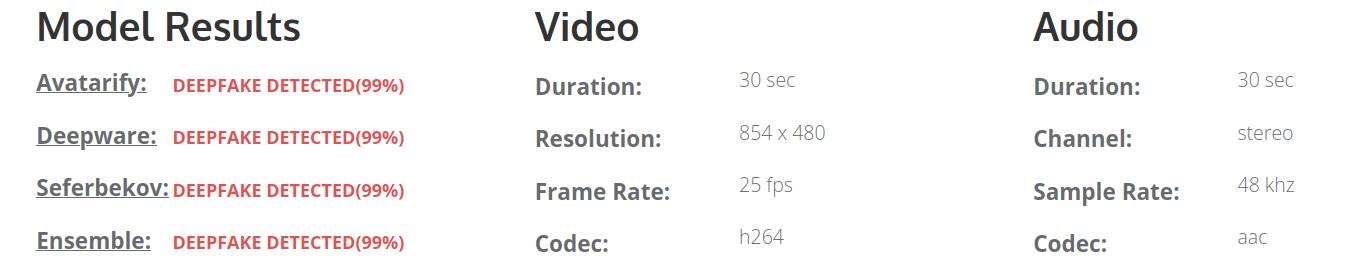
\includegraphics[scale=0.41]{figures/deepware}
	\caption{Overview of the capabilities of Deepware. Screenshot from~\cite{deepware-ai}}\label{fig:deepware}
\end{figure}

A notable feature integrated into Deepware's platform allows for expert
reviews. If mistakes in the deepfake detection process are suspected,
a specialized review can be requested, underscoring the team's commitment
to accuracy and continuous improvement. Deepware also provides a RESTful
\ac{API}\footnote{\url{https://api.deepware.ai}}~\cite{bernarddeepfake}
and \ac{SDK} for developers looking to analyze videos from within
their development setting. Privacy Policy\footnote{\url{https://deepware.ai/privacy-policy/}}
and Terms of Use\footnote{\url{https://deepware.ai/terms-of-services/}} are
also provided by Deepware.

The outcomes of the Detection Accuracy, Precision, Recall and F1-Score assessed
with Deepware are presented in~\autoref{tab:deepware_metrics1} and
in~\autoref{tab:deepware_metrics2}.

\begin{table}[htpb]
	\caption{Computed data using Deepware for calculating evaluation metrics listed in~\autoref{tab:evaluation_metrics}}\label{tab:deepware_metrics1}
	\centering
	\small
	\begin{tabularx}{\textwidth}{>{\centering\arraybackslash}X|>{\centering\arraybackslash}X|>{\centering\arraybackslash}X|>{\centering\arraybackslash}X|>{\centering\arraybackslash}X|>{\centering\arraybackslash}X}
		\cline{1-6}
		\textbf{\#Deepfakes}       & \textbf{\#Genuine videos}  &
		\textbf{\#True Positives}  & \textbf{\#True Negatives}  &
		\textbf{\#False Positives} & \textbf{\#False Negatives}   \\
		\cline{1-6}
		90                         & 20                         &
		85                         & 12                         &
		8                          & 5                            \\
		\cline{1-6}
	\end{tabularx}
\end{table}

\begin{table}[htpb]
	\caption{Computed metrics using Deepware}\label{tab:deepware_metrics2}
	\centering
	\small
	\begin{tabularx}{\textwidth}{>{\centering\arraybackslash}X|>{\centering\arraybackslash}X|>{\centering\arraybackslash}X|>{\centering\arraybackslash}X|>{\centering\arraybackslash}X}
		\cline{1-5}
		\textbf{Processing Time} & \textbf{Detection Accuracy} &
		\textbf{Precision}       & \textbf{Recall}             &
		\textbf{F1-Score}                                        \\
		\cline{1-5}
		Avg. 21,5 sec            & 88,18\%                     &
		91,40\%                  & 94,44\%                     &
		92,9\%                                                   \\
		\cline{1-5}
	\end{tabularx}
\end{table}

\textbf{Detection Accuracy} is the overall correct classification of the tool,
considering both \ac{TP} (deepfakes correctly identified) and \ac{TN}
(genuine videos correctly identified). It is calculated as follows:
\begin{equation}
	{\text{Accuracy}} = \frac{TP + TN}{\textit{Total}} \cdot \textit{100\%}\label{eq:accuracy}
\end{equation}

\textbf{Precision} is the proportion of videos correctly identified as deepfakes
(\ac{TP}) out of all instances (True Positives + \ac{FP}) that the tool classified as deepfakes. It is calculated
as follows:
\begin{equation}
	{\text{Precision}} = \frac{TP}{TP + FP} \cdot \textit{100\%}\label{eq:precision}
\end{equation}

\textbf{Recall} is also known as sensitivity, it is the proportion of True Positives
in relation to the sum of True Positives and \ac{FN}. It is calculated as follows:
\begin{equation}
	{\text{Recall}} = \frac{TP}{TP + FN} \cdot \textit{100\%}\label{eq:recall}
\end{equation}

\textbf{F1-Score} is a metric providing balance between precision and recall, offering
a more comprehensive view of the performance of the tool. It is calculated as follows:
\begin{equation}
	{\text{F1-Score}} = \frac{2 \cdot Precision \cdot Recall}{Precision + Recall}
	= \frac{TP}{TP + \frac{1}{2}(FN + FP)} \cdot \textit{100\%}\label{eq:f1-score}
\end{equation}


One potential drawback of Deepware is the apparent lack of updates since 2021.
This could indicate that no new features or improvements have been introduced
to the tool in recent years, potentially affecting its adaptability to newer
deepfake techniques.


\section{Seferbekov}\label{sec:seferbekov}
Selim Seferbekov's~\cite{seferbekov-github}
deepfake detection tool emerged as a winner in the \ac{DFDC}
challenge, securing a prize of \$500,000~\cite{kaggle2020}. Its acclaim is a testament
to its advanced capabilities and effectiveness in identifying deepfakes.

At its core, Seferbekov's tool operates by examining videos frame-by-frame.
In simpler terms, instead of looking at a video as one whole piece, it
breaks it down and studies each frame just like individual pictures.
This is essential because deepfakes can often differ in quality from one
frame to another.

A major strength of this tool comes from its encoder, the EfficientNet B7~\cite{tan2020efficientnet}.
This encoder is like the brain of the tool and is recognized as one of the
best of its kind. What makes it even more special is that it was trained using
both ImageNet~\cite{ILSVRC15}, a huge database of images, and a method called `noisy student'.
This `noisy student' technique, as detailed in a research paper~\cite{xie2020selftraining},
allows the tool to learn better and improve its accuracy.

For preprocessing, face bounding boxes were extracted using the \ac{MTCNN}~\cite{7553523},
a widely-used method for detecting faces and their landmarks. These bounding boxes
helped determine crop positions, with a margin added around the face to better detect
image noise differences. If multiple faces appeared in a video frame,
the \ac{SSIM}~\cite{1284395} was used to compare the fake and original frames. \ac{SSIM}
measures image differences based on luminance, contrast, and structure. Minimal
differences could change a label from fake to real. The training was done with images
sized 380$\times$380 pixels in batches of 12~\cite{masters-thesis}.

For each video it analyzes, Seferbekov's tool focuses on 32 specific frames.
Rather than just averaging out the results from these frames, a unique
method is employed to analyze them, which has proven to be quite effective.
The tool uses five distinct EfficientNet B7 models, allowing it to analyze content
from multiple perspectives.

However, to run this tool and train it, some powerful computer hardware is needed.
It requires at least four \ac{GPU}s that have a memory
of 12gb or more. If someone is using popular graphics cards like the 1080Ti
or 2080Ti, they might need to adjust some settings to get it working perfectly.

To utilize Seferbekov's detection tool, users need to download the detection
models, add the deepfake videos to the tool's repository, and install certain
Python libraries. In this study, Google Colaboratory was used to test the tool.
The results of the metrics tested are presented in the table below.
Furthermore, the tool is capable of analyzing several videos simultaneously.
Simply group all your deepfake videos in a single folder and provide that
folder as input.

\begin{table}[htpb]
	\caption{Computed data using Seferbekov's tool for calculating evaluation metrics listed in~\autoref{tab:evaluation_metrics}}\label{tab:seferbekov_metrics1}
	\centering
	\small
	\begin{tabularx}{\textwidth}{>{\centering\arraybackslash}X|>{\centering\arraybackslash}X|>{\centering\arraybackslash}X|>{\centering\arraybackslash}X|>{\centering\arraybackslash}X|>{\centering\arraybackslash}X}
		\cline{1-6}
		\textbf{\#Deepfakes}       & \textbf{\#Genuine videos}  &
		\textbf{\#True Positives}  & \textbf{\#True Negatives}  &
		\textbf{\#False Positives} & \textbf{\#False Negatives}   \\
		\cline{1-6}
		90                         & 20                         &
		79                         & 18                         &
		2                          & 11                           \\
		\cline{1-6}
	\end{tabularx}
\end{table}

\begin{table}[htpb]
	\caption{Computed metrics using Seferbekov's tool}\label{tab:seferbekov_metrics2}
	\centering
	\small
	\begin{tabularx}{\textwidth}{>{\centering\arraybackslash}X|>{\centering\arraybackslash}X|>{\centering\arraybackslash}X|>{\centering\arraybackslash}X|>{\centering\arraybackslash}X}
		\cline{1-5}
		\textbf{Processing Time} & \textbf{Detection Accuracy} &
		\textbf{Precision}       & \textbf{Recall}             &
		\textbf{F1-Score}                                        \\
		\cline{1-5}
		Avg. 67,25 sec           & 88,18\%                     &
		97,53\%                  & 87,8\%                      &
		92,41\%                                                  \\
		\cline{1-5}
	\end{tabularx}
\end{table}

The calculations of the Detection Accuracy, Precision, Recall and F1-Score are provided in~\autoref{sec:deepware}.

In terms of interpretability, Seferbekov's tool delivers simple outputs.
Once the detection is complete, it provides users with a \ac{CSV} file detailing the
probability of a video being a deepfake. Its clear output format means users
can quickly grasp the findings. Furthermore, the tool's ability to support
numerous public deepfake datasets highlights its adaptability and relevance in
the field of deepfake detection.

Additionally, Seferbekov's tool is open-source, providing an opportunity
for those with a programming background and knowledge of detection techniques
to modify and extend the implementation to their specific requirements.
This flexibility encourages continuous improvement and adaptability to
emerging deepfake trends.

One potential limitation of Seferbekov's tool is its lack of active support and
usage documentation. This means troubleshooting can be challenging if users
encounter issues. Moreover, the tool's GitHub repository hasn't seen updates
since 2021. Consequently, recent advancements in deepfake techniques might not
be as effectively addressed by this detection tool, potentially impacting its
utility with newer deepfake methods.

\section{NtechLab}
NtechLab's~\cite{ntechlab-github}
software made waves by clinching third place in the \ac{DFDC} Challenge,
walking away with a cool \$100,000 prize~\cite{kaggle2020}. One of the standout
features of this tool is its ability to check multiple deepfake videos
simultaneously. After the analysis, it gives results in a straightforward \ac{CSV}
file, detailing the chances of videos being manipulated.

Before starting with this tool, the necessary training models had to be downloaded.
It should be noted that a decent hardware configuration is essential for the tool
to operate without issues.

While the tool's developers used superior hardware, the decision was made
to work with Google Colaboratory in our research due to the lack of access to such
advanced hardware. This choice highlights the adaptability of the tool
across various platforms.

Talking about the technicalities of how this tool works: the heart of the software is
based on a trio of EfficientNet-B7 models~\cite{tan2020efficientnet}.
These models use Noisy Student~\cite{xie2020selftraining} pre-trained weights.
One of these models looks at video sequences, while the other two break videos
down, frame by frame, changing their approach based on how big the face in the
video is and a few other tweaks.

To make sure the models are spot-on and don't get confused or overdo things,
a special mixup technique was used, alongside some neat tweaks like
AutoAugment~\cite{cubuk2019autoaugment}, Random Erasing~\cite{zhong2017random}
and various video compression parameters~\cite{ntechlab-github}. During training,
video compression was applied in real-time. Short cropped sequences, each
containing 50 frames, were stored in PNG format. In every training cycle, these
sequences were re-encoded with random settings using ffmpeg~\cite{enwiki:1156808546}.
Because of the mixup, the model predictions were `uncertain'. To enhance the model
confidence during inference, a basic transformation was applied. The final
decision was derived by averaging the model's predictions, with weights
based on confidence. The combined time for training and preprocessing was
roughly 5 days on DGX-1~\cite{enwiki:1168440769}.

The NtechLab's tool is open source, which means anyone can access and modify its
code. This allows for greater flexibility, especially for those who wish to
customize or build upon the tool's features. Its open nature encourages
collaboration and adaptation to suit various needs.

The outcomes of the Detection Accuracy, Precision, Recall and F1-Score assessed
with NtechLab's tool are presented in~\autoref{tab:ntechlab_metrics1} and~\autoref{tab:ntechlab_metrics2}.

\begin{table}[htpb]
	\caption{Computed data using NtechLab's tool for calculating evaluation metrics listed in~\autoref{tab:evaluation_metrics}}\label{tab:ntechlab_metrics1}
	\centering
	\small
	\begin{tabularx}{\textwidth}{>{\centering\arraybackslash}X|>{\centering\arraybackslash}X|>{\centering\arraybackslash}X|>{\centering\arraybackslash}X|>{\centering\arraybackslash}X|>{\centering\arraybackslash}X}
		\cline{1-6}
		\textbf{\#Deepfakes}       & \textbf{\#Genuine videos}  &
		\textbf{\#True Positives}  & \textbf{\#True Negatives}  &
		\textbf{\#False Positives} & \textbf{\#False Negatives}   \\
		\cline{1-6}
		90                         & 20                         &
		79                         & 19                         &
		1                          & 11                           \\
		\cline{1-6}
	\end{tabularx}
\end{table}

\begin{table}[htpb]
	\caption{Computed metrics using NtechLab's tool}\label{tab:ntechlab_metrics2}
	\centering
	\small
	\begin{tabularx}{\textwidth}{>{\centering\arraybackslash}X|>{\centering\arraybackslash}X|>{\centering\arraybackslash}X|>{\centering\arraybackslash}X|>{\centering\arraybackslash}X}
		\cline{1-5}
		\textbf{Processing Time} & \textbf{Detection Accuracy} &
		\textbf{Precision}       & \textbf{Recall}             &
		\textbf{F1-Score}                                        \\
		\cline{1-5}
		Avg. 8 min               & 98\%                        &
		98,75\%                  & 87,8\%                      &
		93\%                                                     \\
		\cline{1-5}
	\end{tabularx}
\end{table}

A shared concern with both NtechLab's and Seferbekov's tools is the lack of continuous support
and detailed documentation. While Seferbekov's repository has remained inactive since 2021,
NtechLab's hasn't seen updates since 2020. This stagnation hints at
potential challenges in adapting to the latest deepfake techniques and staying current
in the rapidly advancing realm of deepfake detection.

\section{Facetorch}
Facetorch~\cite{facetorch-github}, crafted by Tomáš Gajarský,
stands out as a tool designed for image forgery detection. It is developed
in Python and PyTorch\footnote{\url{https://pytorch.org/}},
a popular programming framework. It is designed to identify faces and explore the detailed
aspects of facial features using specific algorithms known as neural networks. The aim is to
bring together the finest pre-existing models, enhance their speed with TorchScript\footnote{\url{https://pytorch.org/docs/stable/jit.html}},
and present an all-in-one solution for face analysis. The features it offers include:

\begin{itemize}
	\setlength{\itemsep}{0pt}
	\item Face Detection~\cite{Deng_2020_CVPR}
	\item Facial Representation Learning~\cite{bulat2022pretraining}
	\item Face Verification~\cite{jung2022unified,kim2023adaface}
	\item Facial Expression Recognition~\cite{9582508}
	\item Deepfake Detection~\cite{Luo_2022,seferbekov-github}
	\item 3D Face Alignment~\cite{wu2021synergy}
\end{itemize}

Notably, this tool comes with a user manual~\cite{facetorch}, \ac{API}
instructions~\cite{facetorch-documentation}, and an instance on Hugging Face~\cite{facetorch-hugging-face},
where users benefit from a dedicated interface for deepfake testing. Additionally, for those
familiar with Google Colab, there's a ready-to-use notebook available~\cite{facetorch-google-colab}.
One of its most appealing aspects is its open-source nature, with updates being consistently
rolled out up until March 2023~\cite{facetorch-github}.

The results of the Detection Accuracy, Precision, Recall and F1-Score assessed
with Facetorch are presented in~\autoref{tab:facetorch_metrics1}
and~\autoref{tab:facetorch_metrics2}.

\begin{table}[htpb]
	\caption{Computed data using Facetorch for calculating evaluation metrics listed in~\autoref{tab:evaluation_metrics}}\label{tab:facetorch_metrics1}
	\centering
	\small
	\begin{tabularx}{\textwidth}{>{\centering\arraybackslash}X|>{\centering\arraybackslash}X|>{\centering\arraybackslash}X|>{\centering\arraybackslash}X|>{\centering\arraybackslash}X|>{\centering\arraybackslash}X}
		\cline{1-6}
		\textbf{\#Deepfakes}       & \textbf{\#Genuine videos}  &
		\textbf{\#True Positives}  & \textbf{\#True Negatives}  &
		\textbf{\#False Positives} & \textbf{\#False Negatives}   \\
		\cline{1-6}
		101*                       & 20                         &
		2                          & 20                         &
		0                          & 99                           \\
		\cline{1-6}
	\end{tabularx}
\end{table}

* - Two images couldn't be detected but the overall number of deepfakes is 103 as mentioned in the
last paragraph of~\autoref{sec:analysis-tools}.

\begin{table}[htpb]
	\caption{Computed metrics using Facetorch}\label{tab:facetorch_metrics2}
	\centering
	\small
	\begin{tabularx}{\textwidth}{>{\centering\arraybackslash}X|>{\centering\arraybackslash}X|>{\centering\arraybackslash}X|>{\centering\arraybackslash}X|>{\centering\arraybackslash}X}
		\cline{1-5}
		\textbf{Processing Time} & \textbf{Detection Accuracy} &
		\textbf{Precision}       & \textbf{Recall}             &
		\textbf{F1-Score}                                        \\
		\cline{1-5}
		Avg. 13,5sec             & 18,18\%                     &
		100\%                    & 1,98\%                      &
		3,88\%                                                   \\
		\cline{1-5}
	\end{tabularx}
\end{table}

Based on the results, it's clear that Facetorch had some challenges spotting deepfakes.
One possible explanation is that the way these deepfakes were created might not match well
with the methods the tool uses. Even with this shortcoming in detecting fake images,
the tool still offers valuable information. Not only does it tell us if an image is real or
fake, but it also helps identify the emotions shown in the image, like whether the person
is feeling happy, angry and so on.


\section{Illuminarty}
Illuminarty~\cite{illuminarty-website} is an online platform where users can
easily upload images to detect deepfakes and \ac{AI} generated images~\cite{illuminarty-new-york-times}.
It comes with an \ac{API} option and offers subscription-based plans for those who want to enable more features such as:
\ac{AI} model identification for image generators or unlimited \ac{API} usage. Using the free version,
users can only check \ac{AI} and Deepfake images and texts. There is also a user-friendly Terms of Use\footnote{url{https://illuminarty.ai/en/terms.html}}
and Privacy Policy\footnote{\url{https://illuminarty.ai/en/privacy.html}} sections that explain the tool's purpose and usage instructions.
Additionally, if users need support, they can reach out to the Illuminarty community
through Discord~\cite{illuminarty-discord} or Patreon~\cite{illuminarty-patreon}.

The results of the Detection Accuracy, Precision, Recall and F1-Score assessed
with Illuminarty are presented in~\autoref{tab:facetorch_metrics1} and~\autoref{tab:facetorch_metrics2}.

\begin{table}[htpb]
	\caption{Computed data using Illuminarty for calculating evaluation metrics listed in~\autoref{tab:evaluation_metrics}}\label{tab:illuminarty_metrics1}
	\centering
	\small
	\begin{tabularx}{\textwidth}{>{\centering\arraybackslash}X|>{\centering\arraybackslash}X|>{\centering\arraybackslash}X|>{\centering\arraybackslash}X|>{\centering\arraybackslash}X|>{\centering\arraybackslash}X}
		\cline{1-6}
		\textbf{\#Deepfakes}       & \textbf{\#Genuine videos}  &
		\textbf{\#True Positives}  & \textbf{\#True Negatives}  &
		\textbf{\#False Positives} & \textbf{\#False Negatives}   \\
		\cline{1-6}
		103                        & 20                         &
		26                         & 17                         &
		3                          & 77                           \\
		\cline{1-6}
	\end{tabularx}
\end{table}

\begin{table}[htpb]
	\caption{Computed metrics using Illuminarty}\label{tab:illuminarty_metrics2}
	\centering
	\small
	\begin{tabularx}{\textwidth}{>{\centering\arraybackslash}X|>{\centering\arraybackslash}X|>{\centering\arraybackslash}X|>{\centering\arraybackslash}X|>{\centering\arraybackslash}X}
		\cline{1-5}
		\textbf{Processing Time} & \textbf{Detection Accuracy} &
		\textbf{Precision}       & \textbf{Recall}             &
		\textbf{F1-Score}                                        \\
		\cline{1-5}
		Avg. 3,9sec              & 35\%                        &
		89,7\%                   & 25,24\%                     &
		39,4\%                                                   \\
		\cline{1-5}
	\end{tabularx}
\end{table}

\section{AI or Not}
AI or Not~\cite{aiornot-website} is the idea of Andrey Doronichev,
formerly Director of Product at Google. In 2022 he founded Optic\footnote{\url{https://www.optic.xyz/}},
a startup dedicated to identifying the authenticity of images, videos and voices. Optic offers three
main products:

\textbf{AI or Not}: This tool helps to determine whether an image has been generated by \ac{AI} or a
human.

\textbf{Bias-o-Meter}: This is a smart tool, integrated with the Chrome extension to find hidden biases
and the truth behind the News.

\textbf{NFT fraud detection}: This is tool prevents digital art or \ac{NFT} fraud across blockchains and
marketplaces using real-time detection.

We will be focusing on AI or Not. This tool stands out because of its support and user-friendly guidelines.
To analyze the authenticity of images, you can either upload an image directly to their website or
input an image's web address. While it isn't purely for detecting deepfakes, it's versatile enough
to identify images generated by technologies like Stable Diffusion, MidJourney\footnote{\url{https://www.midjourney.com/}},
DALL-E\footnote{\url{https://openai.com/dall-e-2}} and \ac{GAN}~\cite{ai-or-not}.

The results of the Detection Accuracy, Precision, Recall and F1-Score assessed
with AI or Not are presented in~\autoref{tab:air-or-not_metrics1} and~\autoref{tab:ai-or-not_metrics2}.

\begin{table}[htpb]
	\caption{Computed data using AI or Not for calculating evaluation metrics listed in~\autoref{tab:evaluation_metrics}}\label{tab:air-or-not_metrics1}
	\centering
	\small
	\begin{tabularx}{\textwidth}{>{\centering\arraybackslash}X|>{\centering\arraybackslash}X|>{\centering\arraybackslash}X|>{\centering\arraybackslash}X|>{\centering\arraybackslash}X|>{\centering\arraybackslash}X}
		\cline{1-6}
		\textbf{\#Deepfakes}       & \textbf{\#Genuine videos}  &
		\textbf{\#True Positives}  & \textbf{\#True Negatives}  &
		\textbf{\#False Positives} & \textbf{\#False Negatives}   \\
		\cline{1-6}
		100*                       & 20                         &
		49                         & 20                         &
		0                          & 51                           \\
		\cline{1-6}
	\end{tabularx}
\end{table}

* - Three images couldn't be detected but the overall number of deepfakes is 103 as mentioned in the
last paragraph of~\autoref{sec:analysis-tools}.

\begin{table}[htpb]
	\caption{Computed metrics using AI or Not}\label{tab:ai-or-not_metrics2}
	\centering
	\small
	\begin{tabularx}{\textwidth}{>{\centering\arraybackslash}X|>{\centering\arraybackslash}X|>{\centering\arraybackslash}X|>{\centering\arraybackslash}X|>{\centering\arraybackslash}X}
		\cline{1-5}
		\textbf{Processing Time} & \textbf{Detection Accuracy} &
		\textbf{Precision}       & \textbf{Recall}             &
		\textbf{F1-Score}                                        \\
		\cline{1-5}
		Avg. 3,2sec              & 57,5\%                      &
		100\%                    & 49\%                        &
		65,77\%                                                  \\
		\cline{1-5}
	\end{tabularx}
\end{table}

It also offers Chrome extension and a Telegram bot\footnote{\url{https://t.me/AI_or_not_bot}}, if you
want to stay updated. Your uploaded images are kept private; they've detailed this in their
privacy policy. If you need to test multiple images at once, the documentation guides you on
how to proceed after acquiring \ac{API} access. The tool comfortably supports popular image formats
like JPEG and PNG\@. Privacy Policy\footnote{\url{https://www.aiornot.com/privacy-policy}}
and Terms of Use\footnote{\url{https://www.aiornot.com/terms-of-service}} are also provided by Deepware.

Regarding the interpretability of the output, it tells you if the image is generated by \ac{AI} or Human.
In the words of the creators, AI or Not is a special online tool that quickly tells you if an
image is made by a computer or a person. If the image is made by a computer, the tool
even tells you the exact \ac{AI} method used.


